\documentclass[10pt]{article}

\usepackage[a4paper,margin=1.75cm]{geometry}
\usepackage[T1]{fontenc}
\usepackage[utf8]{inputenc}
\usepackage{lmodern}
\usepackage{microtype}
\usepackage{amsmath,amssymb,amsfonts,mathtools,bm}
\usepackage{booktabs,multirow,array,tabularx,longtable}
\usepackage{enumitem}
\usepackage{graphicx}
\usepackage{xcolor}
\usepackage{tikz}
\usetikzlibrary{arrows.meta,positioning,fit,calc,backgrounds,shapes.geometric,decorations.pathreplacing}
\usepackage{algorithm}
\usepackage{algpseudocode}
\usepackage{listings}
\usepackage{tcolorbox}
\usepackage{hyperref}
\usepackage[nameinlink,capitalise,noabbrev]{cleveref}
\usepackage{natbib}
\usepackage{authblk}
\usepackage{fancyhdr}
\usepackage{titlesec}
\usepackage{caption}
\usepackage{subcaption}
\usepackage{siunitx}

\definecolor{mycgreen}{HTML}{315C3A}
\definecolor{myclight}{HTML}{EAF3EC}
\definecolor{mycgold}{HTML}{9A7626}
\definecolor{mycblue}{HTML}{285A72}
\definecolor{mycred}{HTML}{8A3D3D}
\definecolor{mycgray}{HTML}{5A6468}
\definecolor{codebg}{HTML}{F5F7F6}

\hypersetup{
  colorlinks=true,
  linkcolor=mycblue,
  citecolor=mycgreen,
  urlcolor=mycblue,
  pdftitle={MMALS EcoSpec 1.0},
  pdfauthor={Guillaume Harbonnier}
}

\pagestyle{fancy}
\fancyhf{}
\lhead{MMALS EcoSpec 1.0}
\rhead{Systemic TPUT Specification}
\cfoot{\thepage}
\setlength{\headheight}{14pt}

\titleformat{\section}{\large\bfseries\color{mycgreen}}{\thesection}{0.7em}{}
\titleformat{\subsection}{\normalsize\bfseries\color{mycblue}}{\thesubsection}{0.6em}{}
\titleformat{\subsubsection}{\normalsize\bfseries}{\thesubsubsection}{0.6em}{}

\setlist[itemize]{leftmargin=1.5em,itemsep=2pt,topsep=4pt}
\setlist[enumerate]{leftmargin=1.7em,itemsep=2pt,topsep=4pt}

\newtcolorbox{principlebox}[1][]{
  colback=myclight,
  colframe=mycgreen,
  boxrule=0.7pt,
  arc=1.5mm,
  left=2mm,right=2mm,top=1.5mm,bottom=1.5mm,
  title=#1,
  fonttitle=\bfseries
}
\newtcolorbox{warningbox}[1][]{
  colback=red!3,
  colframe=mycred,
  boxrule=0.7pt,
  arc=1.5mm,
  left=2mm,right=2mm,top=1.5mm,bottom=1.5mm,
  title=#1,
  fonttitle=\bfseries
}
\newtcolorbox{specbox}[1][]{
  colback=blue!2,
  colframe=mycblue,
  boxrule=0.7pt,
  arc=1.5mm,
  left=2mm,right=2mm,top=1.5mm,bottom=1.5mm,
  title=#1,
  fonttitle=\bfseries
}

\lstdefinestyle{pythonstyle}{
  language=Python,
  basicstyle=\ttfamily\footnotesize,
  backgroundcolor=\color{codebg},
  frame=single,
  rulecolor=\color{mycgray!40},
  keywordstyle=\color{mycblue}\bfseries,
  commentstyle=\color{mycgreen},
  stringstyle=\color{mycred},
  breaklines=true,
  showstringspaces=false,
  columns=fullflexible
}

\newcommand{\E}{\mathbb{E}}
\newcommand{\R}{\mathbb{R}}
\newcommand{\D}{\mathcal{D}}
\newcommand{\M}{\mathcal{M}}
\newcommand{\G}{\mathcal{G}}
\newcommand{\A}{\mathcal{A}}
\newcommand{\C}{\mathcal{C}}
\newcommand{\X}{\mathcal{X}}
\newcommand{\Y}{\mathcal{Y}}
\newcommand{\Sset}{\mathcal{S}}
\newcommand{\Rset}{\mathcal{R}}
\newcommand{\Hset}{\mathcal{H}}
\newcommand{\Tr}{\operatorname{Tr}}
\newcommand{\diag}{\operatorname{diag}}
\newcommand{\TopK}{\operatorname{TopK}}
\newcommand{\argmin}{\operatorname*{arg\,min}}
\newcommand{\argmax}{\operatorname*{arg\,max}}

\title{\textbf{MMALS EcoSpec 1.0}\\
\large A Minimal Systemic Architecture for Goal-Conditioned,\\
Memory-Preserving Adaptive Learning}
\author[1]{Guillaume Harbonnier}
\affil[1]{MMALS Project, Independent Research Programme}
\date{June 2026\\\small Conceptual, philosophical, mathematical, and implementation specification}

\begin{document}
\maketitle

\begin{abstract}
Mycelium-Inspired Mutualistic Adaptive Learning Systems (MMALS) began as a modular continual-learning architecture in which specialist hosts exchange transformed latent signals through an adaptive medium. The programme subsequently developed several partially independent branches: latent geometry, energy-guided routing, functional memory, host specialisation, ecosystem audit, goal-conditioned control, reinforcement-learning meta-routing, and forward--backward universal control. The resulting design space is expressive but risks becoming an accumulation of mechanisms rather than an implementable system.

This paper introduces \emph{MMALS EcoSpec 1.0}, a normative system specification that gives these branches one common state model, one minimal operational loop, one objective interface, and one falsification ladder. Its central design rule is: \emph{use the simplest representation and control mechanism that preserves the information required for correct, stable, economical, and auditable action}. The specification distinguishes observation, latent state, context belief, candidate route, committed action, reconstructive memory, synthetic memory, goal, system health, and resource budget. It defines adaptive-complexity modes that range from compiled single-route execution to sparse multi-hypothesis control and critical high-audit operation. It formalises ecosystem-level contribution, functional route memory, goal-conditioned route energy, compression validity, route compilation, and drift-aware fallback. It then maps the same interfaces to the existing RC2O candidate-trace selector, to a contextual-bandit interpretation, to sequential reinforcement learning, and to forward--backward representations for zero-shot control.

EcoSpec is not an empirical claim that the complete architecture outperforms established continual-learning or reinforcement-learning methods. It is an implementation contract and research protocol. Classical probability-simplex routing is the mandatory baseline. Information-geometric and quantum-inspired density-state representations are optional ablations that must earn their additional complexity under controlled cost and parameter budgets. The accompanying repository contains the LaTeX source, an executable Python reference implementation, configuration and trace schemas, contract tests, a smoke demonstration, and a staged experimental roadmap.
\end{abstract}

\noindent\textbf{Keywords:} continual learning, mixture of experts, adaptive routing, energy-based models, goal-conditioned control, reinforcement learning, functional memory, information geometry, system architecture, auditability.

\tableofcontents
\newpage

\section{Introduction}

MMALS was initially motivated by a disciplined biological analogy: a mycelial medium should not merely relay signals, but route, transform, reinforce, prune, and preserve exchanges among heterogeneous hosts. Early prototypes therefore moved from static structural routing to a learnable fungal medium, then to delayed mutualism, soft consolidation, output distillation, functional route memory, and route--function disentanglement. The most important internal result of this sequence is conceptual rather than architectural: preserving a route coefficient vector is not equivalent to preserving the function computed through that route. The relevant memory object is mediated computation, not topology alone \citep{mmalsv09}.

Later branches broadened the programme. Geometry-MMALS asks whether the context--route--host--memory relation forms a stable functional geometry. RC2O provides a transparent candidate-trace selection and continual-learning qualification scaffold. The RL branch treats routing as sequential decision-making under changing goals. Forward--backward control asks whether a reusable representation of reachable futures can support rapid adaptation to new utilities \citep{touati2021learning,touati2022zeroshot}. A quantum-inspired note explores density-state functional memory under ambiguous contexts, while explicitly rejecting any claim of physical quantum advantage \citep{mmalsqi}.

Each branch is individually understandable. The system-level problem is that they can be assembled in too many ways. A design that contains a context estimator, graph geometry, energy model, multiple memories, a router, a meta-policy, a forward model, a backward goal embedding, host-specific transformations, drift diagnostics, and an audit graph may be intellectually rich yet operationally incoherent. A system cannot be implemented, tested, or falsified unless the role, state, interface, and necessity of every mechanism are explicit.

EcoSpec addresses this problem by replacing an additive architecture with a layered contract:

\begin{enumerate}
  \item a \textbf{mandatory minimal kernel} that can be implemented using the current classical MMALS backbone;
  \item \textbf{adaptive mechanisms} that activate only under uncertainty, drift, risk, or goal change;
  \item \textbf{research extensions} that must reduce to the kernel and demonstrate measurable value at controlled cost.
\end{enumerate}

The specification makes six contributions.

\begin{enumerate}
  \item It states six axioms that connect philosophy, mathematics, and engineering.
  \item It defines a complete ecosystem state and a minimal TPUT operational loop.
  \item It formalises goal-conditioned energy routing with adaptive complexity.
  \item It separates reconstructive and synthetic memory and defines safe compilation.
  \item It maps RC2O, RL, and forward--backward control onto one route-decision interface.
  \item It provides a claim ladder, baseline matrix, trace contract, and implementation roadmap.
\end{enumerate}

The term \emph{TPUT} is retained as the established MMALS branch label. This paper treats it as the operational control layer and does not rely on a potentially unstable expansion of the acronym. Its precise meaning is given by the state transition and control contracts in this specification.

\section{Design Problem and Scientific Position}

\subsection{From a host ecology to a complete MMALS ecosystem}

An MMALS host must not be valued only by isolated predictive accuracy, nor only by its relation to other hosts. Its value is its effect on the complete MMALS ecosystem: context inference, routing, transformations, memory, future retention, stability under drift, resource use, auditability, and the final action. The same principle applies to every element of the system.

Let the ecosystem be denoted by
\begin{equation}
  \mathfrak{E} = (\mathcal{O},\mathcal{Z},\mathcal{B},\Hset,\mathcal{T},\Rset,\M^R,\M^S,\mathcal{G},\mathcal{Q},\mathcal{L}),
  \label{eq:ecosystem}
\end{equation}
where the symbols respectively denote observations, latent representation, belief state, hosts, transformations, candidate routes, reconstructive memory, synthetic memory, goals, health/quality state, and audit ledger. A component $e\in\mathfrak{E}$ is useful if its presence improves system-level utility under a declared evaluation protocol.

A simple counterfactual contribution is
\begin{equation}
  \Delta_e = J(\mathfrak{E}) - J(\mathfrak{E}\setminus e),
  \label{eq:counterfactual}
\end{equation}
where $J$ is not accuracy alone, but a declared multi-objective system score. Because interactions matter, pair and coalition effects are also relevant:
\begin{equation}
  \Delta_{e,f}^{\mathrm{int}} = J(\mathfrak{E})-J(\mathfrak{E}\setminus\{e,f\})-\Delta_e-\Delta_f.
  \label{eq:interaction}
\end{equation}
This prevents the mistaken conclusion that a locally weak component is globally useless. A host may stabilise a route, detect ambiguity, provide a low-cost fallback, or preserve an old function even if its standalone accuracy is mediocre.

\subsection{What is preserved and what is allowed to change?}

Continual learning exposes a basic tension. A system must preserve useful old behaviour while adapting to new data. Strong isolation can produce zero forgetting by construction but grows capacity or blocks reuse. Strong sharing improves reuse but exposes old functions to interference. Early MMALS prototypes made this tension explicit, and comparative evaluation must include regularisation, replay, expansion, passive mixture-of-experts, and joint-training controls \citep{kirkpatrick2017overcoming,zenke2017continual,li2017learning,rebuffi2017icarl,lopez2017gradient,rolnick2019experience,rusu2016progressive,mallya2018packnet,shazeer2017outrageously}.

EcoSpec adopts the following position:

\begin{principlebox}[Functional preservation]
MMALS should preserve the function needed by old contexts, not necessarily the exact route, host identity, parameter vector, or internal geometry that previously implemented it.
\end{principlebox}

A route may move while function remains stable; a route may remain fixed while function drifts. Therefore, route stability is a diagnostic but not a sufficient memory criterion.

\subsection{Compression is not commitment}

A common engineering mistake is to equate synthesis with a single label. Let the context posterior be
\begin{equation}
  b_t(c)=q_\omega(c\mid x_t,m_t), \qquad b_t\in\Delta^{C-1}.
\end{equation}
Premature commitment chooses
\begin{equation}
  \hat c_t=\argmax_c b_t(c).
\end{equation}
A compact but uncertainty-preserving synthesis instead stores only the top-$k$ support:
\begin{equation}
  \tilde b_t = \Pi_{k}(b_t), \qquad \|\tilde b_t\|_0\le k,
  \label{eq:topkbelief}
\end{equation}
where $\Pi_k$ renormalises the largest $k$ entries. This can reduce memory and compute without pretending that an ambiguous case is certain.

The operational rule is:

\begin{principlebox}[Compression without premature collapse]
Compress early when information is redundant; commit late when remaining uncertainty could change the action, the safety constraint, the memory update, or the audit conclusion.
\end{principlebox}

\section{Six Normative Axioms}

EcoSpec is governed by six axioms. They are normative engineering rules, not claims about biological mycelium or physical quantum systems.

\subsection{Axiom A1: Systemic Contribution}

\textbf{Statement.} The value of an element is its contribution to the complete MMALS ecosystem under declared goals, constraints, and counterfactual controls.

\textbf{Consequence.} Host specialisation, router quality, memory quality, and geometry quality are measured by system outcomes and interaction effects, not isolated proxies.

\subsection{Axiom A2: Functional Memory}

\textbf{Statement.} The primary memory object is the route-conditioned function required for future behaviour.

For host functions $g_i$, medium transformations $T_i$, and route weights $r_i$, define the mediated latent state
\begin{equation}
  z_f(x,s)=\sum_{i=1}^{H}r_i(x,s)T_i(g_i(x)).
  \label{eq:mediated}
\end{equation}
A functional route record is
\begin{equation}
  \Phi(x,s)=\left\{r_i(x,s),T_i(g_i(x))\right\}_{i=1}^{H},
  \label{eq:functionalroute}
\end{equation}
plus sufficient readout information to reconstruct relevant downstream behaviour.

\subsection{Axiom A3: Deferred Commitment}

\textbf{Statement.} The system preserves a sparse set of relevant hypotheses until an action requires commitment or further uncertainty no longer changes the admissible decision set.

This is not an obligation to execute all hypotheses. It is an obligation not to erase decision-relevant ambiguity solely for implementation convenience.

\subsection{Axiom A4: Sufficient Simplicity}

\textbf{Statement.} MMALS uses the least complex representation and control mechanism that satisfies current requirements for performance, retention, stability, cost, safety, and auditability.

Let $K(r)$ denote route complexity. The route controller solves a constrained problem rather than maximising raw performance:
\begin{align}
  r_t^* \in \argmin_{r\in\Rset_t} \quad & C(r)+\lambda_K K(r) \\
  \text{s.t.}\quad & A(r)\ge A_{\min},\; R(r)\ge R_{\min},\; S(r)\ge S_{\min},\nonumber\\
  & \mathrm{Risk}(r)\le \rho_{\max},\; \mathrm{Audit}(r)\ge q_{\min}.
  \label{eq:confidenceconstrained}
\end{align}
This is the architectural form of ``the minimum cost that buys defensible confidence.''

\subsection{Axiom A5: Goal-Conditioned Control}

\textbf{Statement.} Goals parameterise route evaluation and future control; changing a goal should not require rewriting the architecture.

The default goal vector is
\begin{equation}
  g_t=(w_A,w_R,w_C,w_D,w_S)\in\Delta^4,
  \label{eq:goalvector}
\end{equation}
corresponding to accuracy, retention, cost, drift stability, and ecosystem specialisation. Additional objectives may be appended if their measurement contract is explicit.

\subsection{Axiom A6: Earned Complexity and Falsifiable Reduction}

\textbf{Statement.} Every advanced mechanism must reduce to a simpler baseline and must demonstrate incremental value under matched resource and parameter budgets.

Examples include:
\begin{itemize}
  \item multi-hypothesis routing must reduce to top-1 routing;
  \item RL control must reduce to one-step energy selection;
  \item information geometry must reduce to Euclidean/simplex diagnostics;
  \item density-state memory must reduce to diagonal probabilistic routing;
  \item compiled memory must fall back to reconstructive execution when its validity envelope fails.
\end{itemize}

\section{Complete Ecosystem State}

\subsection{State tuple}

At decision time $t$, the operational state is
\begin{equation}
  s_t = (x_t,z_t,b_t,\Gamma_t,\mu_t^R,\mu_t^S,g_t,h_t,\beta_t,\ell_t),
  \label{eq:state}
\end{equation}
with:
\begin{itemize}
  \item $x_t\in\X$: raw or preprocessed observation;
  \item $z_t=f_\phi(x_t)\in\mathcal{Z}$: shared perceptual representation;
  \item $b_t\in\Delta^{C-1}$: context belief;
  \item $\Gamma_t$: current route/host/memory graph;
  \item $\mu_t^R$: reconstructive memory state;
  \item $\mu_t^S$: synthetic or compiled memory state;
  \item $g_t$: goal vector or utility descriptor;
  \item $h_t$: system-health vector, including drift and calibration;
  \item $\beta_t$: compute, latency, energy, memory, and risk budgets;
  \item $\ell_t$: audit and claim-ledger state.
\end{itemize}

The state is intentionally broader than an RL environment state. It includes epistemic and governance variables needed to decide how much complexity is justified.

\subsection{Route object}

A candidate route $\varrho\in\Rset_t$ is a typed object:
\begin{equation}
  \varrho=(\tilde b,\mathcal{I},\bm r,\mathcal{T},\mathcal{K},\mathcal{M},\mathcal{O}),
  \label{eq:routeobject}
\end{equation}
where:
\begin{itemize}
  \item $\tilde b$ is the context support used by the route;
  \item $\mathcal{I}\subseteq\{1,\ldots,H\}$ is the active host set;
  \item $\bm r$ contains host or path allocations;
  \item $\mathcal{T}$ identifies transformations;
  \item $\mathcal{K}$ identifies a coalition or execution graph;
  \item $\mathcal{M}$ declares memory retrieval and update operations;
  \item $\mathcal{O}$ declares readout and action semantics.
\end{itemize}

The route is more than a probability vector. It is an executable proposal with predicted cost, risk, memory consequences, and audit depth.

\subsection{Typed host interface}

Each host $H_i$ exposes
\begin{equation}
  H_i: (z_t,\xi_i)\mapsto (u_i,\kappa_i,q_i),
\end{equation}
where $u_i$ is a representation or proposal, $\kappa_i$ is execution cost, and $q_i$ is a quality/health report. Hosts may be trainable models, frozen perceptual groves, symbolic solvers, retrieval modules, human-expert channels, or external services. A mature sensory grove is therefore part of the ecosystem even when it is not an adaptive host in the same parameter-update regime.

\subsection{System health}

A minimal health vector is
\begin{equation}
  h_t=(d_z,d_r,d_y,d_T,d_J,\mathrm{ECE},\mathrm{OOD},\mathrm{load},\mathrm{age}),
  \label{eq:health}
\end{equation}
containing latent drift, route drift, output drift, transformation drift, Jacobian/local-sensitivity drift, calibration error, out-of-distribution score, resource load, and memory age. Not every deployment computes every term. The selected health representation itself follows Axiom A4.

\section{The Minimal TPUT Operational Loop}

\begin{figure*}[t]
\centering
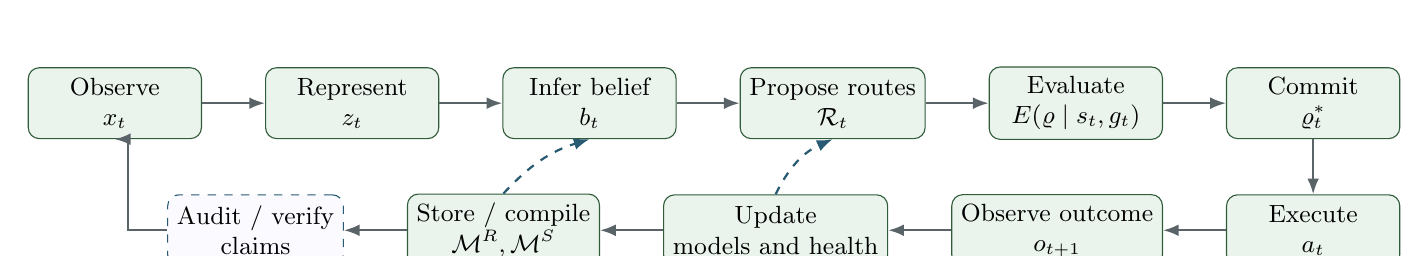
\begin{tikzpicture}[
  node distance=7mm and 8mm,
  box/.style={draw=mycgreen,rounded corners,fill=myclight,minimum height=9mm,minimum width=22mm,align=center,font=\small},
  opt/.style={draw=mycblue,rounded corners,dashed,fill=blue!2,minimum height=9mm,minimum width=22mm,align=center,font=\small},
  arrow/.style={-{Latex[length=2mm]},thick,mycgray}
]
\node[box] (observe) {Observe\\$x_t$};
\node[box,right=of observe] (represent) {Represent\\$z_t$};
\node[box,right=of represent] (belief) {Infer belief\\$b_t$};
\node[box,right=of belief] (propose) {Propose routes\\$\Rset_t$};
\node[box,right=of propose] (evaluate) {Evaluate\\$E(\varrho\mid s_t,g_t)$};
\node[box,right=of evaluate] (commit) {Commit\\$\varrho_t^*$};
\node[box,below=of commit] (execute) {Execute\\$a_t$};
\node[box,left=of execute] (outcome) {Observe outcome\\$o_{t+1}$};
\node[box,left=of outcome] (update) {Update\\models and health};
\node[box,left=of update] (memory) {Store / compile\\$\M^R,\M^S$};
\node[opt,left=of memory] (audit) {Audit / verify\\claims};

\draw[arrow] (observe)--(represent);
\draw[arrow] (represent)--(belief);
\draw[arrow] (belief)--(propose);
\draw[arrow] (propose)--(evaluate);
\draw[arrow] (evaluate)--(commit);
\draw[arrow] (commit)--(execute);
\draw[arrow] (execute)--(outcome);
\draw[arrow] (outcome)--(update);
\draw[arrow] (update)--(memory);
\draw[arrow] (memory)--(audit);
\draw[arrow] (audit.west) -- ++(-5mm,0) |- (observe.south);
\draw[arrow,dashed,mycblue] (memory.north) to[bend left=15] (belief.south);
\draw[arrow,dashed,mycblue] (update.north) to[bend left=20] (propose.south);
\end{tikzpicture}
\caption{The mandatory TPUT loop. Optional mechanisms change how belief, route proposal, evaluation, and memory are implemented; they do not change the contract between stages.}
\label{fig:tputloop}
\end{figure*}

The minimal loop in \cref{fig:tputloop} contains ten stages.

\begin{enumerate}
  \item \textbf{Observe}: acquire $x_t$ and metadata.
  \item \textbf{Represent}: compute $z_t$ using a perceptual adapter.
  \item \textbf{Infer belief}: update context belief $b_t$ without compulsory top-1 collapse.
  \item \textbf{Propose}: generate a bounded candidate set $\Rset_t$.
  \item \textbf{Evaluate}: compute energy, constraints, and predicted future effects.
  \item \textbf{Commit}: select a route or safe abstention.
  \item \textbf{Execute}: run the route and produce action/output.
  \item \textbf{Observe outcome}: collect labels, delayed effects, or environment transitions.
  \item \textbf{Update}: update permitted parameters, health, and control estimates.
  \item \textbf{Store/compile/audit}: append reconstructive evidence, update synthetic memory, and verify claims.
\end{enumerate}

The simplest valid implementation may use a frozen encoder, a softmax context estimator, a finite candidate list, a linear energy score, a top-1 route, a supervised loss, and JSON audit records. RL, graph geometry, density matrices, or dynamic topology are not required to satisfy the base specification.

\begin{algorithm}[t]
\caption{EcoSpec inference and action}
\label{alg:inference}
\begin{algorithmic}[1]
\Require observation $x_t$, ecosystem state $s_{t-1}$, goal $g_t$, budget $\beta_t$
\State $z_t\gets\textsc{Perceive}(x_t)$
\State $b_t\gets\textsc{InferContext}(z_t,\mu_{t-1}^R,\mu_{t-1}^S)$
\State $m_t\gets\textsc{SelectComplexityMode}(b_t,h_{t-1},\beta_t)$
\State $\Rset_t\gets\textsc{ProposeRoutes}(z_t,b_t,m_t,\Gamma_{t-1})$
\ForAll{$\varrho\in\Rset_t$}
  \State $(E_\varrho,c_\varrho,v_\varrho)\gets\textsc{EvaluateRoute}(\varrho,s_{t-1},g_t)$
\EndFor
\State $\varrho_t^*\gets\textsc{CommitOrAbstain}(\Rset_t,E,c,v)$
\State $(y_t,a_t,\tau_t)\gets\textsc{Execute}(\varrho_t^*,x_t)$
\State \Return $(y_t,a_t,\tau_t)$
\end{algorithmic}
\end{algorithm}

\section{Adaptive Complexity: Simple by Default, Rich When Required}

\subsection{Three operating modes}

EcoSpec defines three mandatory modes, each of which may have multiple implementation profiles.

\begin{table}[h]
\centering
\caption{Adaptive-complexity modes.}
\label{tab:modes}
\begin{tabularx}{\textwidth}{lXXX}
\toprule
Mode & Entry condition & Representation/control & Memory/audit \\
\midrule
Fast & low uncertainty, valid compiled route, low drift/risk & top-1 or narrow top-$k$; deterministic energy selection & synthetic memory; compact trace \\
Ambiguous & competing contexts/routes or moderate drift & sparse belief and route set; optional coalition execution & mixed retrieval; comparative trace \\
Critical & high risk, OOD, hard retention constraint, regulation, or failed validity envelope & expanded candidates, hard constraints, conservative policy, abstention or human gate & reconstructive memory; full evidence trace \\
\bottomrule
\end{tabularx}
\end{table}

A mode selector can use entropy, energy gap, drift, and risk:
\begin{align}
  u_t &= H(b_t),\\
  \delta_t &= E_{(2)}-E_{(1)},\\
  \chi_t &= \alpha_u u_t + \alpha_d d_t + \alpha_r \mathrm{Risk}_t - \alpha_g\delta_t.
  \label{eq:complexityscore}
\end{align}
Thresholds $(\theta_F,\theta_C)$ select fast, ambiguous, or critical mode. This rule is deliberately simple; it can later become a learned policy.

\subsection{A compression invariance condition}

Let $E(\varrho\mid s)$ be the full route energy and $\tilde E(\varrho\mid\tilde s)$ the energy computed from a compressed state. Suppose
\begin{equation}
  |E(\varrho\mid s)-\tilde E(\varrho\mid\tilde s)|\le\epsilon
  \quad\forall\varrho\in\Rset.
  \label{eq:uniformerror}
\end{equation}

\textbf{Proposition 1 (ranking preservation).} If the energy gap between the best and second-best full-state routes is greater than $2\epsilon$, compression preserves the selected route.

\textit{Proof.} Let $\varrho_1$ and $\varrho_2$ be the best and second-best full-state routes. Then
$E(\varrho_2)-E(\varrho_1)>2\epsilon$. In the worst case, compression raises $\varrho_1$ by $\epsilon$ and lowers $\varrho_2$ by $\epsilon$, leaving $\tilde E(\varrho_2)>\tilde E(\varrho_1)$. \hfill$\square$

This proposition supplies a practical compilation test: strong route margin permits aggressive compression; weak margin triggers a richer mode.

\subsection{Deferred commitment as action-set dominance}

Given context belief $b$ and utility $U(a,c)$, the Bayes action is
\begin{equation}
  a_B=\argmax_{a\in\A}\sum_c b(c)U(a,c).
\end{equation}
A MAP-context controller selects $\hat c=\argmax_c b(c)$ and then
\begin{equation}
  a_M=\argmax_a U(a,\hat c).
\end{equation}
Because $a_M\in\A$, Bayes optimality gives
\begin{equation}
  \sum_c b(c)U(a_B,c)\ge \sum_c b(c)U(a_M,c).
\end{equation}
The result is elementary but important: preserving the belief does not guarantee perfect decisions, yet it cannot be intrinsically worse than forcing the controller to act as though the MAP context were certain, when both have access to the same action set and utility model.

\section{Goal-Conditioned Energy Routing}

\subsection{Route energy}

EcoSpec uses energy as the common comparison language between supervised selection, policy control, and constrained optimisation \citep{lecun2006tutorial}. For route $\varrho$, state $s$, and goal $g$, define
\begin{align}
E_\theta(\varrho\mid s,g) = {}&
  w_A \widehat L_{\mathrm{task}}(\varrho)
 +w_R \widehat L_{\mathrm{ret}}(\varrho)
 +w_C \widehat C(\varrho) \\
&+w_D \widehat D(\varrho)
 +w_K \widehat K(\varrho)
 +w_Q \widehat Q_{\mathrm{risk}}(\varrho) \\
&-w_S \widehat U_{\mathrm{spec}}(\varrho)
 -w_M \widehat U_{\mathrm{mut}}(\varrho)
 -w_A^{\mathrm{audit}}\widehat U_{\mathrm{audit}}(\varrho).
\label{eq:energy}
\end{align}
Terms are normalised to declared ranges before weighting. The five primary goal weights in \cref{eq:goalvector} map to groups of these terms. Hard requirements are not converted into arbitrary soft weights; they remain constraints.

A stochastic router is
\begin{equation}
  p_\theta(\varrho\mid s,g)=
  \frac{\exp(-E_\theta(\varrho\mid s,g)/\tau)}
  {\sum_{\varrho'\in\Rset}\exp(-E_\theta(\varrho'\mid s,g)/\tau)}.
  \label{eq:boltzmann}
\end{equation}
The fast mode takes $\argmin E$. Ambiguous mode retains top-$k$ routes. Critical mode may reject all routes if no candidate satisfies hard constraints.

\subsection{Mutualistic and systemic contribution}

For a route using host $i$, the local leave-one-out gain is
\begin{equation}
  G_i = L(\varrho\setminus i)-L(\varrho).
\end{equation}
Positive $G_i$ means the host improves the current route. EcoSpec extends this to a system objective:
\begin{equation}
  G_i^{\mathrm{sys}} = J_{t:t+T}(\mathfrak E)-J_{t:t+T}(\mathfrak E\setminus H_i),
  \label{eq:systemgain}
\end{equation}
which can include retention, cost, drift, and future option value. Because exact counterfactuals are expensive, implementation may use periodic ablations, doubly robust estimators, Shapley approximations, or route swaps. The estimator and its uncertainty must be recorded.

\subsection{Complexity regularisation}

A route complexity term may be
\begin{equation}
  K(\varrho)=\alpha_H |\mathcal{I}|+\alpha_E|E_\varrho|+\alpha_M M_{\mathrm{bytes}}+\alpha_L\mathrm{latency}+\alpha_T\mathrm{traceDepth}.
  \label{eq:routecomplexity}
\end{equation}
The purpose is not to reward small models unconditionally. It is to prevent unearned complexity from masquerading as intelligence.

\section{Dual Memory: Reconstructive and Synthetic}

\subsection{Reconstructive memory}

Reconstructive memory $\M^R$ stores the evidence required to reproduce or contest a decision. A normative trace includes:
\begin{itemize}
  \item observation reference and feature/version hashes;
  \item context posterior and uncertainty diagnostics;
  \item candidate routes and rejection reasons;
  \item goal vector, hard constraints, and budgets;
  \item route energies and component terms;
  \item selected route, host coalition, transformations, and model versions;
  \item outcome, delayed feedback, and memory update;
  \item claim-verification status and provenance.
\end{itemize}

Reconstructive memory can be expensive. Its retention policy is risk- and governance-dependent.

\subsection{Synthetic memory}

Synthetic memory $\M^S$ stores reusable abstractions:
\begin{itemize}
  \item context and function prototypes;
  \item compiled macro-routes;
  \item low-rank route/geometry summaries;
  \item calibrated energy surrogates;
  \item policy/value states;
  \item validity envelopes and fallback pointers.
\end{itemize}

A compiled route $\kappa$ is valid only inside an envelope
\begin{equation}
  \mathcal V_\kappa=(\mathcal Z_\kappa,\mathcal G_\kappa,\mathcal H_\kappa,\mathcal B_\kappa,\delta_\kappa,\epsilon_\kappa),
  \label{eq:envelope}
\end{equation}
covering latent support, allowed goals, health regime, budgets, drift tolerance, and maximum estimated regret.

\subsection{Compilation criterion}

A candidate macro-route is compiled when
\begin{align}
  n_\kappa &\ge n_{\min},\\
  \widehat{\mathrm{Regret}}(\kappa)&\le\epsilon_{\max},\\
  \widehat{\mathrm{Drift}}(\kappa)&\le\delta_{\max},\\
  \mathrm{AuditRecoverability}(\kappa)&\ge a_{\min},\\
  \mathrm{CostGain}(\kappa)&\ge c_{\min}.
\end{align}
Compilation is therefore a measured transformation from reconstructive evidence to a cheaper reusable policy, not an irreversible deletion of history.

\begin{figure}[h]
\centering
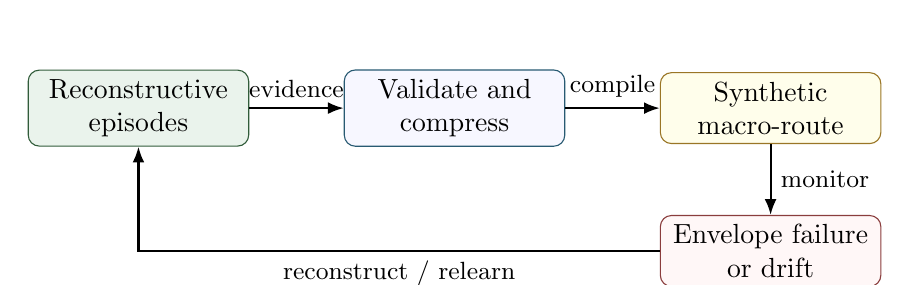
\begin{tikzpicture}[
 node distance=9mm and 12mm,
 b/.style={draw,rounded corners,align=center,minimum width=28mm,minimum height=9mm},
 a/.style={-{Latex[length=2mm]},thick}
]
\node[b,fill=myclight,draw=mycgreen] (rich) {Reconstructive\\episodes};
\node[b,right=of rich,fill=blue!3,draw=mycblue] (learn) {Validate and\\compress};
\node[b,right=of learn,fill=yellow!8,draw=mycgold] (compiled) {Synthetic\\macro-route};
\node[b,below=of compiled,fill=red!3,draw=mycred] (fallback) {Envelope failure\\or drift};
\draw[a] (rich)-- node[above,font=\small]{evidence} (learn);
\draw[a] (learn)-- node[above,font=\small]{compile} (compiled);
\draw[a] (compiled)-- node[right,font=\small]{monitor} (fallback);
\draw[a] (fallback.west) -| node[pos=0.25,below,font=\small]{reconstruct / relearn} (rich.south);
\end{tikzpicture}
\caption{Synthetic memory is a reversible compilation layer over reconstructive evidence.}
\label{fig:memory}
\end{figure}

\section{Geometry of the MMALS State}

\subsection{Mandatory classical geometry}

The classical state has a product structure
\begin{equation}
  \mathcal S = \mathcal Z\times\Delta^{C-1}\times\Delta^{R-1}\times\mathcal M\times\mathcal G\times\mathcal H.
  \label{eq:productgeometry}
\end{equation}
Euclidean latent distance is not sufficient for every factor. Probability-simplex variables admit divergences and information-geometric metrics \citep{amari2016information}. A practical block metric is
\begin{equation}
  d^2(s,s')=
  \lambda_z\|z-z'\|_2^2+
  \lambda_c d_{\mathrm{JS}}^2(b,b')+
  \lambda_r d_{\mathrm{JS}}^2(p_r,p_r')+
  \lambda_h\|h-h'\|_{W_h}^2.
  \label{eq:blockmetric}
\end{equation}
This geometry can support nearest prototypes, drift detection, route continuity, and local trust regions. It does not by itself establish causal specialisation.

\subsection{Route graph and transport}

Let $\Gamma_t=(V_t,E_t)$ be a typed graph whose vertices may include contexts, hosts, transformations, memory objects, and outputs. Edge attributes encode allocation, cost, confidence, and age. A route is a typed path or small subgraph. Continual update can be interpreted as transport of functional state over $\Gamma_t$, constrained by memory and health.

Geometry-G1 questions whether learned routes exhibit functional mediation rather than only nominal clustering. EcoSpec places this question at the diagnostic layer: route continuity, perturbation maps, candidate permutations, route swaps, and held-out contexts determine whether geometry is operationally meaningful.

\subsection{Optional density-state extension}

For ambiguous contexts, a quantum-inspired extension may represent route-function state using a positive semidefinite trace-one matrix
\begin{equation}
  \rho\succeq 0,\qquad \Tr(\rho)=1.
  \label{eq:density}
\end{equation}
Classical routing is the diagonal case
\begin{equation}
  \rho_R=\diag(r_1,\ldots,r_H).
\end{equation}
Off-diagonal terms encode learned pairwise coherence or interaction, not physical quantum entanglement. A low-rank implementation can use
\begin{equation}
  \rho=\frac{UU^\top}{\Tr(UU^\top)}.
\end{equation}
The extension is admissible only if it improves performance, memory diagnostics, calibration, or cost-normalised robustness beyond diagonal routing and ordinary covariance/Gram alternatives \citep{stoudenmire2016supervised,schuld2019quantum,mmalsqi}. It remains a research branch, not part of the mandatory kernel.

\section{Continual Update and Functional Preservation}

\subsection{Drift decomposition}

EcoSpec distinguishes at least five drifts:
\begin{align}
D_r &= \E\|r_{\mathrm{cur}}-r_{\mathrm{ref}}\|_2^2,\\
D_z &= \E\|z_{f,\mathrm{cur}}-z_{f,\mathrm{ref}}\|_2^2,\\
D_y &= \E D_{\mathrm{KL}}(p_{\mathrm{ref}}\|p_{\mathrm{cur}}),\\
D_T &= \E\sum_i \omega_i\|T_{i,\mathrm{cur}}(g_i(x))-T_{i,\mathrm{ref}}(g_i(x))\|_2^2,\\
D_J &= \E\sum_i \omega_i\|J_{i,\mathrm{cur}}-J_{i,\mathrm{ref}}\|_F^2.
\end{align}
Route-only preservation can yield $D_r\approx0$ while $D_z$ and $D_y$ remain large. Co-evolution experiments further ask whether $D_T$ or $D_J$ contributes explanatory value beyond $D_r,D_z,D_y$ \citep{mmalsv012}.

\subsection{Update objective}

A generic continual update is
\begin{align}
\mathcal L_t = {}& \mathcal L_{\mathrm{new}}
+\lambda_rD_r+\lambda_zD_z+\lambda_yD_y
+\lambda_TD_T+\lambda_JD_J\\
&+\lambda_E\mathcal L_{\mathrm{energy}}
+\lambda_H H(p_r)+\lambda_C C(\varrho)
+\lambda_Q\mathcal L_{\mathrm{constraints}}.
\label{eq:continualobjective}
\end{align}
Only terms supported by the active implementation profile are enabled. Coefficients must be validation-selected, and every enabled term requires an ablation.

\subsection{Continual update algorithm}

\begin{algorithm}[h]
\caption{Continual update with functional memory}
\label{alg:update}
\begin{algorithmic}[1]
\Require new experience batch $B_t$, reconstructive memory $\M^R$, synthetic memory $\M^S$
\State retrieve old-context anchors $B_{\mathrm{old}}$ under memory budget
\State compute new-task loss and current route/function states
\State compute enabled drift terms against frozen references
\State apply hard safety and parameter-update masks
\State optimise permitted parameters
\State evaluate all seen contexts using frozen protocol
\State update health, calibration, and claim ledger
\State append reconstructive trace
\State test compilation, invalidation, and fallback conditions
\end{algorithmic}
\end{algorithm}

\section{RC2O Correspondence}

RC2O is treated as the current transparent candidate-trace selection and continual-learning qualification backbone. EcoSpec does not replace it. It defines the target interfaces that allow RC2O evidence to become a system-control layer.

\begin{table}[h]
\centering
\caption{RC2O-to-EcoSpec correspondence.}
\label{tab:rc2o}
\begin{tabularx}{\textwidth}{p{0.27\textwidth}X}
\toprule
RC2O object & EcoSpec interpretation \\
\midrule
Candidate trace & Executable route candidate $\varrho$ with features and provenance \\
Metric evaluator & Measurement map for accuracy, retention, cost, stability, specialisation, and audit \\
Protocol verifier & Hard constraints, dataset split, seed policy, evaluation timing, and leakage checks \\
Claim verifier & Claim ledger mapping evidence to allowed, blocked, or provisional claims \\
Selected candidate & Committed route, policy, or model configuration \\
Regime detector & Context belief and health state $(b_t,h_t)$ \\
Eight-dataset scaffold & Offline ecosystem-state and candidate-route benchmark \\
Goal A--E & Goal vector $g=(w_A,w_R,w_C,w_D,w_S)$ \\
Post-hoc retention evaluation & Delayed transition utility and functional-memory audit \\
Trace row / CSV artifact & Reconstructive memory record and machine-readable audit event \\
\bottomrule
\end{tabularx}
\end{table}

The RC2O selector can be expressed as a one-step EcoSpec decision:
\begin{equation}
  \varrho^*=\argmin_{\varrho\in\Rset(s)}E(\varrho\mid s,g).
  \label{eq:rc2oselector}
\end{equation}
If candidate consequences do not affect future state, this is a contextual bandit. If route selection changes host specialisation, memory, drift, or future candidate availability, the problem is sequential and requires RL or model-predictive control.

\subsection{Adapter contract}

An RC2O adapter must provide:
\begin{enumerate}
  \item state extraction from existing metric and diagnostic rows;
  \item candidate conversion into typed route objects;
  \item goal-conditioned scoring;
  \item protocol and claim constraint evaluation;
  \item selected-candidate logging in the trace schema;
  \item delayed outcome ingestion for RL extension.
\end{enumerate}

The accompanying repository implements a minimal adapter around dictionary/CSV-like candidate rows.

\section{Reinforcement-Learning Extension}

\subsection{MDP and constrained control view}

When route decisions have delayed consequences, define an MDP or POMDP
\begin{equation}
  (\Sset,\A,P,R_g,\gamma),
\end{equation}
where state is the ecosystem state, action is a route/configuration decision, and transition includes learning, memory, host load, and drift. The goal-conditioned reward is
\begin{equation}
  R_g(s,a,s')=-E(a\mid s,g)-\lambda_{\mathrm{viol}}V(s,a,s').
  \label{eq:rlreward}
\end{equation}
A policy $\pi_\psi(a\mid s,g)$ can then learn long-horizon trade-offs \citep{sutton2018reinforcement,haarnoja2018soft}.

The one-step energy router is recovered when $\gamma=0$ or when actions have no relevant delayed effect. Thus RL is an extension, not a competing architecture.

\subsection{Why route selection is genuinely sequential}

Selecting a host changes the data it receives. That changes its future competence. Selecting a synthetic macro-route may reduce audit depth. Repeatedly choosing a dominant host can suppress specialisation elsewhere. Updating a route can protect or damage old functions. Consequently, the controller helps create the ecosystem it later observes.

A minimal transition model is
\begin{equation}
  s_{t+1}=F_\eta(s_t,a_t,o_{t+1})+\varepsilon_t.
\end{equation}
The RL branch is justified only when a multi-step policy improves declared metrics relative to one-step energy selection under the same candidate set and budget.

\subsection{Safe policy hierarchy}

EcoSpec recommends a policy hierarchy:
\begin{enumerate}
  \item hard constraints and safety shield;
  \item compiled policy if its validity envelope holds;
  \item deterministic energy controller;
  \item learned RL policy within the admissible action set;
  \item abstention or human gate if no action is admissible.
\end{enumerate}
This ordering prevents a high-capacity policy from bypassing the system contract.

\section{Forward--Backward Universal Control Correspondence}

Forward--backward (FB) representations learn reusable factors of successor occupancy so that policies for new rewards can be obtained without retraining from scratch \citep{touati2021learning,touati2022zeroshot}. In a simplified notation,
\begin{equation}
  M^{\pi_z}(s,a,s^+)\approx F(s,a,z)^\top B(s^+).
  \label{eq:fb}
\end{equation}
The backward representation embeds future states or reward support; the forward representation describes route-conditioned reachable occupancy.

EcoSpec maps this structure as follows:
\begin{itemize}
  \item $s$: MMALS ecosystem state;
  \item $a$: route or coalition decision;
  \item $F(s,a,z)$: reachable future ecosystem effects under a latent control intent;
  \item $B(s^+)$: backward embedding of desired future state, constraint satisfaction, or utility;
  \item $z_g$: latent control code derived from the current goal vector;
  \item $\pi_{z_g}$: zero-shot or rapidly adapted route policy.
\end{itemize}

A conceptual FB route score is
\begin{equation}
  Q_g(s,a)\approx F(s,a,z_g)^\top z_g,
  \label{eq:fbscore}
\end{equation}
or, with an explicit desired future distribution $\nu_g$,
\begin{equation}
  z_g=\E_{s^+\sim\nu_g}[B(s^+)].
\end{equation}
The controller then selects an admissible action with maximal predicted goal alignment.

\begin{figure}[h]
\centering
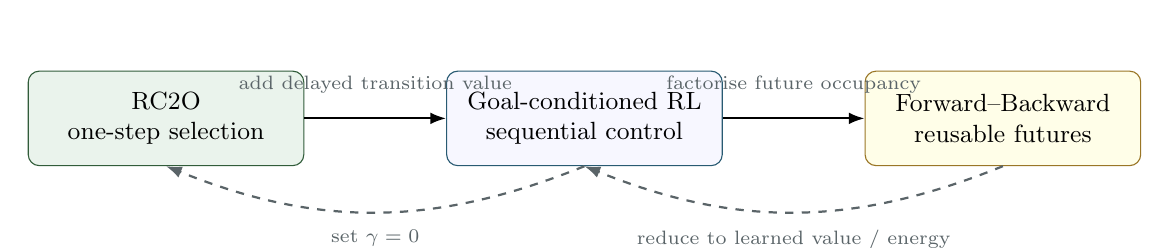
\begin{tikzpicture}[
 node distance=10mm and 18mm,
 b/.style={draw,rounded corners,align=center,minimum width=35mm,minimum height=12mm,font=\small},
 a/.style={-{Latex[length=2mm]},thick}
]
\node[b,fill=myclight,draw=mycgreen] (rc) {RC2O\\one-step selection};
\node[b,right=of rc,fill=blue!3,draw=mycblue] (rl) {Goal-conditioned RL\\sequential control};
\node[b,right=of rl,fill=yellow!9,draw=mycgold] (fb) {Forward--Backward\\reusable futures};
\draw[a] (rc)--(rl);
\draw[a] (rl)--(fb);
\node[font=\scriptsize,mycgray,above=2mm of $(rc)!0.5!(rl)$] {add delayed transition value};
\node[font=\scriptsize,mycgray,above=2mm of $(rl)!0.5!(fb)$] {factorise future occupancy};
\draw[a,dashed,mycgray] (fb.south) to[bend left=22] node[below=1mm,font=\scriptsize]{reduce to learned value / energy} (rl.south);
\draw[a,dashed,mycgray] (rl.south) to[bend left=22] node[below=1mm,font=\scriptsize]{set $\gamma=0$} (rc.south);
\end{tikzpicture}
\caption{RC2O, RL, and FB are successive control profiles over the same typed route action.}
\label{fig:controlprofiles}
\end{figure}

Soft FB generalises the class of utilities and provides a useful future comparison, but it is not a required component of EcoSpec \citep{bagatella2026softfb}. The first implementation milestone is a transparent sequential meta-router, not zero-shot universal control.

\section{Implementation Contract}

\subsection{Module boundaries}

The reference implementation uses the following interfaces:

\begin{table}[h]
\centering
\caption{Normative module contracts.}
\label{tab:interfaces}
\begin{tabularx}{\textwidth}{lXX}
\toprule
Module & Input & Output \\
\midrule
Perceptor & observation & latent vector and quality metadata \\
Context model & latent, memories, health & context belief and uncertainty \\
Route proposer & state, mode & bounded candidate route set \\
Energy model & state, goal, route & energy decomposition and constraint report \\
Controller & evaluated candidates & committed route or abstention \\
Executor & route, observation & output/action and execution trace \\
Memory manager & trace, outcome & reconstructive append, synthetic update, invalidations \\
Health monitor & state, outcome & drift/calibration/load state \\
Claim verifier & metrics, protocol & claim status and evidence pointers \\
RC2O adapter & candidate rows & typed routes and outcomes \\
RL adapter & transitions & policy/value update \\
\bottomrule
\end{tabularx}
\end{table}

\subsection{Reference data classes}

The package defines immutable or validated data classes for goals, context beliefs, route candidates, energy breakdowns, trace records, and ecosystem state. The controller must never infer missing constraint semantics from field names. Every metric declares direction, scale, and provenance.

\subsection{Feature flags}

The default configuration disables research extensions:
\begin{itemize}
  \item single-step deterministic energy control enabled;
  \item sparse multi-hypothesis context enabled only above uncertainty threshold;
  \item synthetic compilation enabled with conservative envelope checks;
  \item RL disabled;
  \item forward--backward control disabled;
  \item information-geometric metric optional;
  \item density-state memory disabled.
\end{itemize}

\subsection{Trace schema}

Every decision trace has a stable identifier and references:
\begin{equation}
  \tau_t=(\mathrm{id},t,x,z,b,g,h,\beta,\Rset,E,c,\varrho^*,a,o,\Delta\M,\mathrm{claims}).
\end{equation}
The repository includes a JSON Schema. Production implementations may split sensitive observation references from the audit record while preserving integrity hashes.

\section{Experimental Programme and Falsification Ladder}

\subsection{Stage 0: contract validation}

Before model training, test:
\begin{itemize}
  \item route probabilities and context beliefs are normalised;
  \item hard constraints cannot be bypassed by energy weights;
  \item a compiled route invalidates outside its envelope;
  \item goal changes alter route ranking in a controlled toy system;
  \item deterministic runs reproduce traces under fixed seeds;
  \item optional profiles reduce to the classical kernel.
\end{itemize}

\subsection{Stage 1: frozen-backbone route control}

Use fixed perceptual features and a frozen host bank. This isolates context, route, goal, memory, and audit behaviour from representation learning. Required demonstrations:
\begin{enumerate}
  \item route changes under goals A--E;
  \item each change improves its target metric or satisfies its constraint;
  \item complexity mode changes at declared uncertainty/drift thresholds;
  \item synthetic routes fall back correctly.
\end{enumerate}

\subsection{Stage 2: RC2O offline trace benchmark}

Use the RC2O eight-dataset scaffold as an offline decision dataset. Compare:
\begin{itemize}
  \item fixed weighted score;
  \item goal-conditioned linear energy;
  \item nonlinear energy model;
  \item contextual bandit;
  \item oracle selected by future outcomes.
\end{itemize}
The key metric is not only selected accuracy, but regret against the best admissible candidate under each goal.

\subsection{Stage 3: continual-learning backbone}

Integrate the selected EcoSpec controller with the current RC2O continual-learning backbone. Mandatory baselines include fine-tuning, EWC, SI, LwF, replay, PNN, sparse MoE, and joint training. Hyperparameters are validation-selected, not arbitrary defaults. Report final average accuracy, forgetting, minimum-task accuracy, backward transfer, memory, latency, training time, parameter count, and GPU memory.

\subsection{Stage 4: sequential meta-routing}

Construct an environment where current route choice changes future host competence, cost, or retention. Compare deterministic energy selection, contextual bandit, RL, and model-predictive control. RL earns inclusion only if long-horizon utility improves without violating constraints.

\subsection{Stage 5: forward--backward control}

After the environment and RL transition model are stable, test whether FB representations allow rapid goal switching without per-goal retraining. Compare against goal-conditioned value networks and successor-feature baselines.

\subsection{Stage 6: advanced geometry ablations}

Only after the classical system is stable, test:
\begin{itemize}
  \item Fisher/JS geometry versus Euclidean diagnostics;
  \item covariance/Gram state versus density-state memory;
  \item real low-rank state versus complex amplitude state;
  \item diagonal versus off-diagonal route-state models.
\end{itemize}
An advanced representation is rejected if gains disappear under parameter, memory, and compute matching.

\subsection{Claim ladder}

\begin{table}[h]
\centering
\caption{Claim ladder and minimum evidence.}
\label{tab:claims}
\begin{tabularx}{\textwidth}{lX}
\toprule
Claim level & Minimum evidence \\
\midrule
C0 -- Executable specification & contract tests, deterministic smoke trace, schema validation \\
C1 -- Functional memory & route/function ablation; functional drift aligns with forgetting better than route drift \\
C2 -- Goal-responsive control & route changes across goals and improves goal-specific utility under constraints \\
C3 -- Sequential control value & RL/MPC improves long-horizon utility over one-step energy \\
C4 -- Geometry value & geometric metrics improve prediction/control beyond ordinary baselines \\
C5 -- Density-state value & off-diagonal/low-rank state improves cost-matched ambiguous-context performance or diagnosis \\
C6 -- General MMALS advantage & multi-benchmark, multi-seed, hardened baselines, external replication \\
\bottomrule
\end{tabularx}
\end{table}

\section{Relationship to Prior MMALS Versions}

\begin{longtable}{p{0.14\textwidth}p{0.31\textwidth}p{0.46\textwidth}}
\caption{Research-line mapping into EcoSpec.}\label{tab:history}\\
\toprule
Branch/version & Main lesson & EcoSpec location \\
\midrule
\endfirsthead
\toprule
Branch/version & Main lesson & EcoSpec location \\
\midrule
\endhead
v0.1--v0.2 & structural preservation can reduce interference, but isolation and capacity controls are necessary & route object, complexity cost, baseline and claim ladder \\
v0.3--v0.4 & the medium needs its own cost/utility; immediate mutualistic pressure can destabilise learning & energy decomposition, delayed activation, system contribution \\
v0.5--v0.7 & output and latent preservation matter; specialisation alone is not memory & functional memory axiom and dual-memory update \\
v0.8--v0.9 & separate mechanistic from performance claims; route identity is not function & drift decomposition and claim C1 \\
v0.11 & broad comparative harness and cost metrics & stage-3 baseline hardening \\
v0.12--v0.13 & transformation geometry may co-drift; stronger regularisation can over-constrain plasticity & health vector, optional drift terms, earned complexity \\
v1.x inferred context & explicit task identity must be replaced by latent context belief and guarded routing & state $b_t$, deferred commitment, complexity modes \\
RC2O & transparent candidate selection, continual qualification, evidence trace & RC2O adapter and one-step controller \\
Geometry-G1 & test functional route mediation, continuity, perturbation, and held-out validity & product geometry and geometry claim C4 \\
TPUT & goal-conditioned operational loop, dual memory, safe control & full EcoSpec kernel \\
RL/Universal Control & sequential route decisions and goal switching & RL and FB control profiles \\
QI & mixed route-function memory under ambiguity & optional density-state extension \\
\bottomrule
\end{longtable}

\section{Risks, Non-Claims, and Design Failure Modes}

\begin{warningbox}[Scientific non-claims]
EcoSpec does not claim that MMALS solves continual learning, that the mycelium analogy is causal, that geometry automatically improves control, that density matrices imply quantum advantage, or that the full architecture should be enabled in one implementation.
\end{warningbox}

Major failure modes include:
\begin{enumerate}
  \item \textbf{Architecture inflation}: every research branch is enabled at once.
  \item \textbf{Proxy capture}: route entropy or host dominance is mistaken for useful specialisation.
  \item \textbf{Goal laundering}: arbitrary weights produce a desired ranking without validated metric scales.
  \item \textbf{Audit theatre}: traces record values but not versions, provenance, or rejected candidates.
  \item \textbf{Compiled-memory lock-in}: cheap macro-routes continue after drift invalidates them.
  \item \textbf{RL overreach}: sequential control is added where one-step selection is sufficient.
  \item \textbf{Geometry decoration}: elaborate manifolds do not improve prediction, control, or diagnosis.
  \item \textbf{Baseline weakness}: poorly tuned EWC, replay, PNN, or MoE artificially inflates MMALS value.
  \item \textbf{Hidden capacity}: gains arise from more parameters, memory, or compute.
  \item \textbf{Irreversible ambiguity loss}: early top-1 context selection removes the information needed for safe action.
\end{enumerate}

The correct response to a failed advanced branch is reduction, not rhetorical rescue. The classical kernel remains the control.

\section{Discussion}

EcoSpec gives MMALS coherence by treating geometry, energy, memory, specialisation, audit, and control as views of one decision process rather than as independent modules. Geometry describes the state and its neighbourhoods. Energy compares admissible routes under a goal. Memory preserves reconstructive evidence and compiles recurrent functions. Specialisation is an ecosystem contribution pattern. Audit records why a route was admissible and why a claim is allowed. RL extends the same route decision across time. Forward--backward representations seek reusable descriptions of reachable futures.

The design is intentionally asymmetric: the simplest classical route is normative; advanced state representations are hypotheses. This asymmetry is necessary. An architecture cannot be ``keep it simple'' if every conceptual insight becomes a mandatory layer. Simplicity must be encoded in the objective, the mode selector, the reduction tests, and the claim process.

The deepest implication is that abstraction and uncertainty preservation are compatible. MMALS does not need to keep every raw detail in active memory. It can compress observations into latent states, prune beliefs to sparse support, compile repeated route-functions, and reuse macro-policies. What it must preserve is the information capable of changing action, adaptation, or audit. Compression is therefore judged by decision and reconstruction error, not by fidelity to every historical detail.

\section{Conclusion}

MMALS EcoSpec 1.0 transforms a broad research programme into an implementable system contract. It defines the ecosystem state, the minimal TPUT loop, adaptive complexity, goal-conditioned energy, dual memory, functional preservation, RC2O correspondence, RL extension, and forward--backward control path. It preserves the current MMALS backbone rather than replacing it. It also gives every advanced branch a reduction test and a falsification gate.

The central system principle is:

\begin{principlebox}[EcoSpec design rule]
Keep the architecture simple; allow behaviour to become complex only when uncertainty, risk, drift, memory, or the goal requires it.
\end{principlebox}

A system that follows this rule can maintain multiple possibilities without carrying unlimited detail, compile repeated experience without losing fallback, and change objectives without retraining its entire architecture. The next scientific step is not another conceptual layer. It is implementation of the classical kernel, contract validation, integration with RC2O traces, and controlled evidence that each additional mechanism earns its cost.

\appendix
\section{Notation Summary}

\begin{longtable}{p{0.17\textwidth}p{0.72\textwidth}}
\toprule
Symbol & Meaning \\
\midrule
$x_t$ & observation at time $t$ \\
$z_t$ & perceptual latent state \\
$b_t$ & context belief distribution \\
$\Gamma_t$ & typed ecosystem graph \\
$H_i,g_i$ & host and host representation function \\
$T_i$ & medium transformation for host $i$ \\
$\varrho$ & executable route candidate \\
$\Rset_t$ & candidate route set \\
$z_f$ & mediated latent exchange \\
$g_t$ & goal vector \\
$h_t$ & system health vector \\
$\beta_t$ & resource/risk budget \\
$E(\varrho\mid s,g)$ & goal-conditioned route energy \\
$\M^R,\M^S$ & reconstructive and synthetic memory \\
$D_r,D_z,D_y,D_T,D_J$ & route, functional latent, output, transformation, and Jacobian drift \\
$\rho$ & optional positive semidefinite route-function state \\
$F,B$ & forward and backward representations in FB control \\
\bottomrule
\end{longtable}

\section{Normative Pseudocode for Compilation}

\begin{algorithm}[h]
\caption{Synthetic-memory compilation and invalidation}
\begin{algorithmic}[1]
\Require reconstructive episodes $\mathcal E_\kappa$, thresholds $n_{\min},\epsilon,\delta,a_{\min},c_{\min}$
\If{$|\mathcal E_\kappa|<n_{\min}$}
  \State \Return not compiled
\EndIf
\State fit candidate macro-route $\kappa$
\State estimate regret, drift, audit recoverability, and cost gain by held-out episodes
\If{all thresholds pass}
  \State create validity envelope $\mathcal V_\kappa$
  \State store $\kappa$ in $\M^S$ with fallback pointers to $\M^R$
\Else
  \State retain reconstructive execution only
\EndIf
\For{each execution of $\kappa$}
  \If{state outside $\mathcal V_\kappa$ or monitored drift exceeds threshold}
    \State invalidate $\kappa$ and fall back to reconstructive route proposal
  \EndIf
\EndFor
\end{algorithmic}
\end{algorithm}

\section{Minimal Repository Acceptance Criteria}

A release satisfies EcoSpec 1.0 when:
\begin{enumerate}
  \item the paper compiles without errors;
  \item the Python package installs locally;
  \item contract tests pass;
  \item the toy demonstration shows at least two goals selecting different routes;
  \item invalid routes are rejected by hard constraints;
  \item a trace validates against the JSON schema;
  \item RC2O-like candidate rows can be adapted and scored;
  \item optional RL and density-state flags default to disabled;
  \item README, version, citation, and licence files are present.
\end{enumerate}

\section{Example Goal Profiles}

\begin{table}[h]
\centering
\caption{Illustrative goal profiles; production weights require calibration.}
\begin{tabular}{lccccc}
\toprule
Profile & Accuracy & Retention & Cost & Stability & Specialisation \\
\midrule
A: accuracy & 0.60 & 0.15 & 0.05 & 0.15 & 0.05 \\
B: retention & 0.20 & 0.55 & 0.05 & 0.15 & 0.05 \\
C: low cost & 0.20 & 0.10 & 0.55 & 0.10 & 0.05 \\
D: drift stability & 0.20 & 0.20 & 0.05 & 0.50 & 0.05 \\
E: ecosystem specialisation & 0.20 & 0.15 & 0.05 & 0.10 & 0.50 \\
\bottomrule
\end{tabular}
\end{table}

\begin{thebibliography}{99}

\bibitem[Amari(2016)]{amari2016information}
S. Amari.
\newblock \emph{Information Geometry and Its Applications}.
\newblock Springer, 2016.

\bibitem[Bagatella et~al.(2026)Bagatella, Rupf, Martius, and Krause]{bagatella2026softfb}
M. Bagatella, T. Rupf, G. Martius, and A. Krause.
\newblock Soft forward--backward representations for zero-shot reinforcement learning with general utilities.
\newblock arXiv:2602.06769, 2026.

\bibitem[Fedus et~al.(2022)Fedus, Zoph, and Shazeer]{fedus2022switch}
W. Fedus, B. Zoph, and N. Shazeer.
\newblock Switch transformers: Scaling to trillion parameter models with simple and efficient sparsity.
\newblock \emph{Journal of Machine Learning Research}, 23(120):1--39, 2022.

\bibitem[Haarnoja et~al.(2018)Haarnoja, Zhou, Abbeel, and Levine]{haarnoja2018soft}
T. Haarnoja, A. Zhou, P. Abbeel, and S. Levine.
\newblock Soft actor-critic: Off-policy maximum entropy deep reinforcement learning with a stochastic actor.
\newblock In \emph{ICML}, pages 1861--1870, 2018.

\bibitem[Kirkpatrick et~al.(2017)Kirkpatrick et~al.]{kirkpatrick2017overcoming}
J. Kirkpatrick et~al.
\newblock Overcoming catastrophic forgetting in neural networks.
\newblock \emph{Proceedings of the National Academy of Sciences}, 114(13):3521--3526, 2017.

\bibitem[LeCun et~al.(2006)LeCun, Chopra, Hadsell, Ranzato, and Huang]{lecun2006tutorial}
Y. LeCun, S. Chopra, R. Hadsell, M. Ranzato, and F. J. Huang.
\newblock A tutorial on energy-based learning.
\newblock In \emph{Predicting Structured Data}. MIT Press, 2006.

\bibitem[Li and Hoiem(2018)]{li2017learning}
Z. Li and D. Hoiem.
\newblock Learning without forgetting.
\newblock \emph{IEEE TPAMI}, 40(12):2935--2947, 2018.

\bibitem[Lopez-Paz and Ranzato(2017)]{lopez2017gradient}
D. Lopez-Paz and M. Ranzato.
\newblock Gradient episodic memory for continual learning.
\newblock In \emph{NeurIPS}, 2017.

\bibitem[Mallya and Lazebnik(2018)]{mallya2018packnet}
A. Mallya and S. Lazebnik.
\newblock PackNet: Adding multiple tasks to a single network by iterative pruning.
\newblock In \emph{CVPR}, pages 7765--7773, 2018.

\bibitem[MMALS Project(2026a)]{mmalsv09}
MMALS Project.
\newblock MMALS Prototype 0.9: Route--Function Disentanglement and Functional Memory Validation.
\newblock Internal research report, May 2026.

\bibitem[MMALS Project(2026b)]{mmalsv011}
MMALS Project.
\newblock MMALS Prototype 0.11: Comparative Evidence Harness.
\newblock Internal research report, May 2026.

\bibitem[MMALS Project(2026c)]{mmalsv012}
MMALS Project.
\newblock MMALS Prototype 0.12: Hopfield / Co-Evolution Branch.
\newblock Internal research report, May 2026.

\bibitem[MMALS Project(2026d)]{mmalsqi}
MMALS Project.
\newblock MMALS-QI: A Quantum-Inspired Extension of Mycelium-Inspired Mutualistic Adaptive Learning Systems.
\newblock Internal research note, May 2026.

\bibitem[Rebuffi et~al.(2017)Rebuffi, Kolesnikov, Sperl, and Lampert]{rebuffi2017icarl}
S.-A. Rebuffi, A. Kolesnikov, G. Sperl, and C. H. Lampert.
\newblock iCaRL: Incremental classifier and representation learning.
\newblock In \emph{CVPR}, pages 2001--2010, 2017.

\bibitem[Rolnick et~al.(2019)Rolnick, Ahuja, Schwarz, Lillicrap, and Wayne]{rolnick2019experience}
D. Rolnick, A. Ahuja, J. Schwarz, T. Lillicrap, and G. Wayne.
\newblock Experience replay for continual learning.
\newblock In \emph{NeurIPS}, 2019.

\bibitem[Rusu et~al.(2016)Rusu et~al.]{rusu2016progressive}
A. A. Rusu et~al.
\newblock Progressive neural networks.
\newblock arXiv:1606.04671, 2016.

\bibitem[Schuld and Killoran(2019)]{schuld2019quantum}
M. Schuld and N. Killoran.
\newblock Quantum machine learning in feature Hilbert spaces.
\newblock \emph{Physical Review Letters}, 122:040504, 2019.

\bibitem[Shazeer et~al.(2017)Shazeer et~al.]{shazeer2017outrageously}
N. Shazeer et~al.
\newblock Outrageously large neural networks: The sparsely-gated mixture-of-experts layer.
\newblock In \emph{ICLR}, 2017.

\bibitem[Stoudenmire and Schwab(2016)]{stoudenmire2016supervised}
E. M. Stoudenmire and D. J. Schwab.
\newblock Supervised learning with quantum-inspired tensor networks.
\newblock In \emph{NeurIPS}, 2016.

\bibitem[Sutton and Barto(2018)]{sutton2018reinforcement}
R. S. Sutton and A. G. Barto.
\newblock \emph{Reinforcement Learning: An Introduction}.
\newblock MIT Press, second edition, 2018.

\bibitem[Touati and Ollivier(2021)]{touati2021learning}
A. Touati and Y. Ollivier.
\newblock Learning one representation to optimize all rewards.
\newblock In \emph{NeurIPS}, 2021.

\bibitem[Touati et~al.(2022)Touati, Rapin, and Ollivier]{touati2022zeroshot}
A. Touati, J. Rapin, and Y. Ollivier.
\newblock Does zero-shot reinforcement learning exist?
\newblock arXiv:2209.14935, 2022.

\bibitem[Zenke et~al.(2017)Zenke, Poole, and Ganguli]{zenke2017continual}
F. Zenke, B. Poole, and S. Ganguli.
\newblock Continual learning through synaptic intelligence.
\newblock In \emph{ICML}, pages 3987--3995, 2017.

\end{thebibliography}

\end{document}
